
\newpage
\section{Model package}

In questa sezione descriveremo il package \textbf{Model}.

Questo package contiene le implementazioni dei concetti che riguardano
la pi\`u importante e ricca astrazione del concetto di vertice, del
nostro modello di grafo, delle specializzazioni del concetto di
vertice e di due astrazioni legate alla programmazione funzionale.

\subsection{Supplied Abstractions}

Le astrazioni fornite da questo package sono le seguenti:
\begin{itemize}
\label{itemize:model-supplied-abstraction}
\item fornire l'astrazione di vertice e le sue specializzazioni
  necessarie per implementare gli altri moduli del progetto. Questa
  astrazione pu\`o essere modellata a livello teorico come un
  \emph{abstract data type}, in quanto non siamo interessati che i
  client siano a conoscenza delle specifiche realizzazioni (come
  invece lo sarebbe se fosse stato un \emph{algebraic data type}), ma
  vogliamo usare un approccio trasparente per mantenere flessibile il
  sistema. Le specializzazioni del concetto di vertice che ho
  implementato riguardo il concetto semplice di vertice, di vertice da
  usare in una ricerca \emph{DFS} e nell'algoritmo di Tarjan per la
  ricerca delle componenti fortemente connesse.
\item fornire l'astrazione del grafo, arricchendola con comportamenti
  per poter modificare la struttura del grafo rappresentato e poter
  eseguire delle computazioni su di esso: \`e possibile usare due idee
  prese dal paradigma funzionale per agire sui vertici del grafo ed
  \`e fornita una implementazione dell'algoritmo \emph{DFS}, che espone
  degli \emph{hot spots} in modo da permettere ai client di avere
  gi\`a implementata la struttura dell'algoritmo, fornendo solo il
  comportamento specifico di interesse.
\item nascondere tutti i tipi che implementano i concetti astratti ai
  client di questo package, in modo da utilizzare le astrazioni
  mediante interfaccie e non accoppiando i client con specifiche
  realizzazioni attraverso delle factory 
\item interfacciare le astrazioni di vertice e grafo con gli oggetti
  definiti nel package \emph{DotInterface}, per permettere una
  rappresentazione grafica che cattura le idee definite nell'articolo
  \cite{tellingStories}
\end{itemize}

\subsection{Class diagram}

Non \`e possibile visualizzare tutte le classi implementate in questo
package in un unico diagramma di classe, per maggior chiarezza le
raggruppo in diagrammi pi\`u piccoli, cercando come fatto nelle
descrizioni degli altri package, di rappresentare e commentare gli
aspetti pi\`u importanti.

\subsubsection{Vertex and OurModel}
Il diagramma rappresentato in figura
\ref{fig:vertex-abstraction-interfaces} rappresenta le interfaccie
dei concetti fondamentali del progetto, quelli di vertice e del nostro
modello di grafo. Commento le interfaccie in paragrafi indipendenti:

\begin{figure}
  \centering
  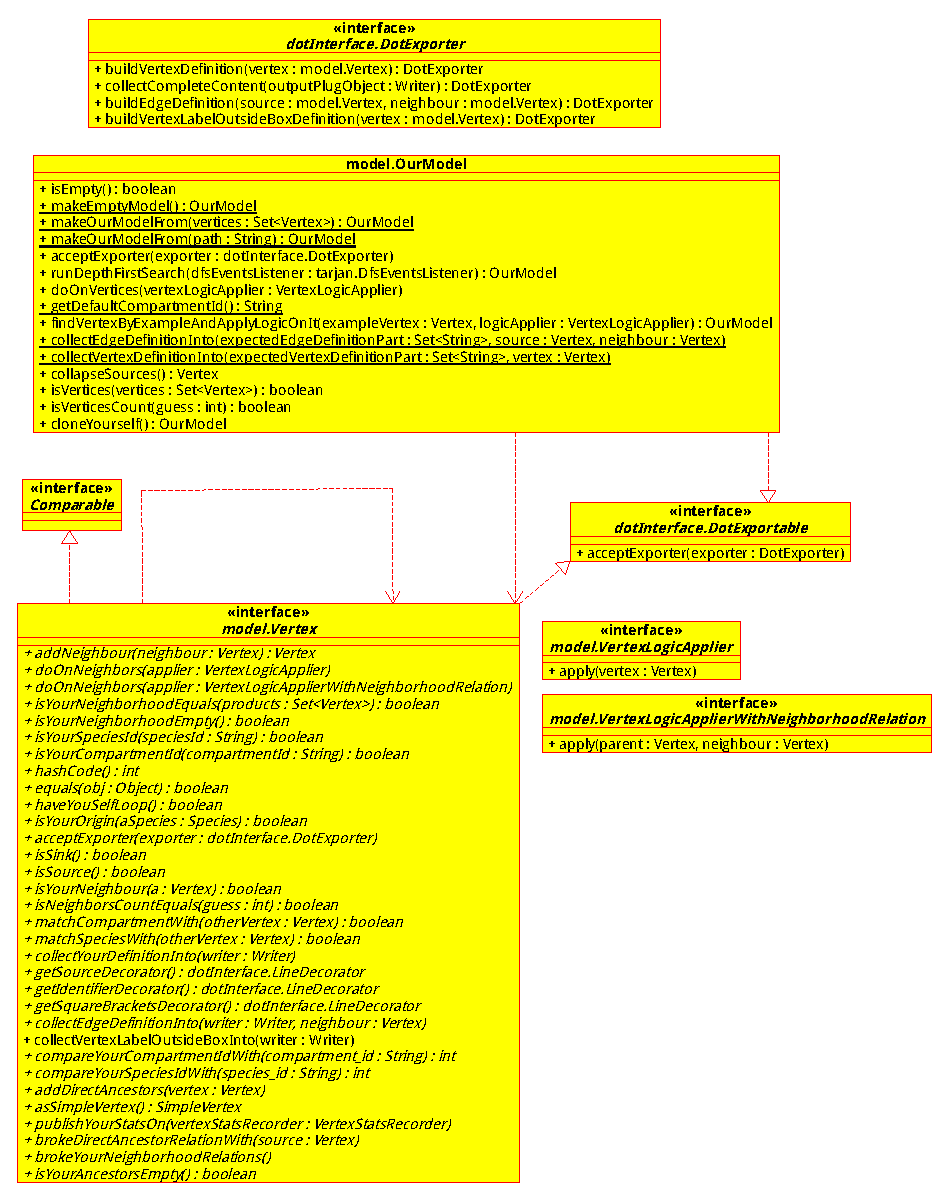
\includegraphics{packages/vertex-interface-class-diagram.eps}
  \caption{Vertex abstraction interfaces}
  \label{fig:vertex-abstraction-interfaces}
\end{figure}

\begin{paragraph}{Vertex}

L'interfaccia \emph{Vertex} cattura queste idee:
\begin{itemize}
\item aggiungere informazioni sul vicinato di un vertice, dando la
  possibilit\`a sia di aggiungere vicini che predecessori (quindi
  modelliamo sia una lista di adiacenza, sia una lista di incidenza)
\item fornire informazioni sulle caratteristiche del vertice, ad
  esempio se un vertice \`e sorgente o pozzo, qual \`e il suo
  vicinato, quali sono le informazioni che lo distinguono (riferite
  alle informazioni sulla specie e sul compartment recuperate dal
  modello SBML di origine)
\item dare la possibilit\`a di "rompere" le proprie relazioni di
  vicinato per permettere una compattazione delle sorgenti in una
  unica.
\item accettare un esportatore per costruire un documento .dot,
  fornendo gli oggetti necessari per la corretta formattazione delle
  informazioni incapsulate nell'oggetto vertice.
\item forzare la riscrittura dei metodi \emph{equals} and
  \emph{hashCode} in modo che tutte le implementazioni di questa
  interfaccia possano essere trattati come \emph{value objects}, non
  distinguendoli per riferimento in memoria, bensi dalle informazioni
  che questi incapsulano.
\item poter applicare della logica sul vicinato utilizzando uno stile
  preso dalla programmazione funzionale, catturato dalle interfaccie
  \emph{VertexLogicApplier} e la sua variante che permette di lavorare
  sulla coppia \emph{(source, neighbor)}.
\item imporre una relazione d'ordine totale fra oggetti che
  implementano questa interfaccia, in modo da rendere gli algoritmi
  deterministici nel momento di selezione di vertici. Questo \`e stato
  utile per la stesura dei metodi di unit testing.
\end{itemize}
\end{paragraph}

\begin{paragraph}{OurModel}
La classe concreta \emph{OurModel} cattura queste idee:
\begin{itemize}
\item catturare il concetto di grafo da utilizzare come modello di
  dominio per le computazioni che descriver\`o nel seguito di questo
  documento.
\item fornire il comportamento per la costruzione del modello in
  diverse modalit\`a: costruire un modello vuoto da riempire
  successivamente, oppure a partire da un modello SBML
\item implementare la logica per compattare le sorgenti in una unica
\item applicare della logica fornita da un generico client su tutti i
  vertici, utilizzando l'idea funzionale descritta nella descrizione
  dell'interfaccia \emph{Vertex}
\item implementare un \emph{template} della ricerca \emph{DFS} usando
  \emph{hook methods} per specializzare la ricerca relativamente alle
  necessit\`a del client di questa classe.
\end{itemize}
\end{paragraph}

\subsubsection{Vertex implementors}
\begin{figure}
  \centering
  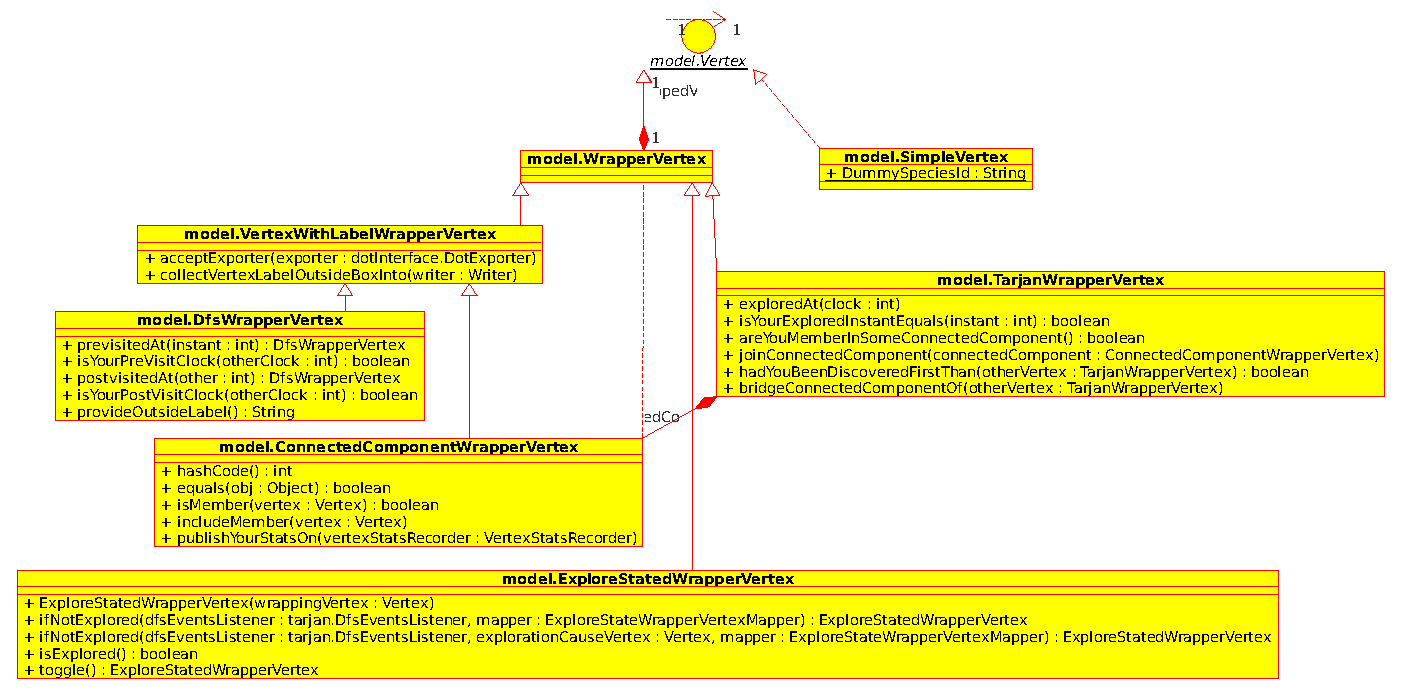
\includegraphics[angle=90]{packages/vertex-implementors.eps}
  \caption{Vertex implementors}
  \label{fig:vertex-implementors}
\end{figure}
fd